%\section{Implementation of the Framework}
Due to the limited time-frame of this project, we aimed to evaluate the usability of our proposed framework, rather than creating a complete implementation thereof.
Hence, we focused on creating a program, which allows us to simulate a fully functional implementation of the framework, in order to conduct realistic experiments.
Our framework should allow an inexperienced user to construct action models in PDDL that can be used in a goal-oriented approach.
The actions are learned by demonstration and then used to execute complex tasks such as the permutation of objects on the table.

%We evaluated the usability of this framework in terms of experiments discussed in Chapter \ref{Evaluation}.
Consider the PbD principle overview shown in \fig{fig:Baxter-Case-Study}.
By iterating through the individual stages, we implemented our framework with the following functionalities:
\begin{itemize}
\item Search for an object,
\item Record a simple movement which represents the action,
\item Assign predicates and parameters to the learned action,
\item Create the action model in PDDL,
\item Execute a sequence of created actions defined in an external file.
\end{itemize}

  \begin{figure}[ht]
    \centering
    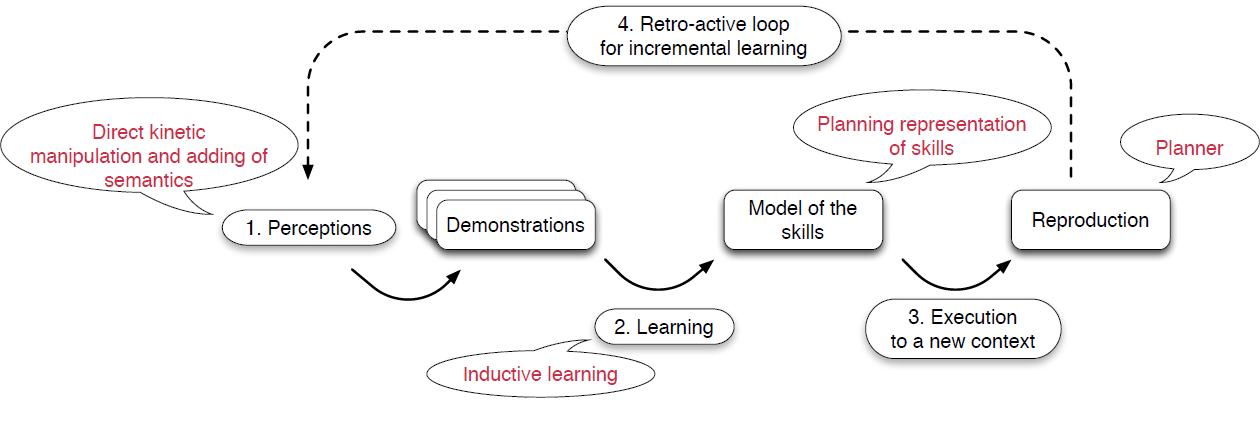
\includegraphics[scale=0.45]{figures/Baxter-Case-Study}
    \caption{PbD principle overview}
    \label{fig:Baxter-Case-Study}
  \end{figure}

%This framework allows the user to create any actions needed for the PDDL domain.
In the following sections we will discuss the implementation of each of the above mentioned functionalities in depth.

%\subsection{Intera Software}
%The industrial version of the Baxter robot currently comes with the Intera 3 software that provides a graphical user interface.
The software allows the selection of the basic tasks in order to build an action sequence.
Aimed at taking over factory operations that usually employ several people, the industrial version of Baxter can easily be taught simple tasks without the need for programming.


%%%% Step 1 %%%%
\section{Baxter Research Robot}
We implemented the framework using a Baxter Research Robot (\cite{robotics2013baxter}), which is required to learn the action models needed for a pick-and-place action.
Baxter is a two-armed humanoid robot created by Rethink Robotics and introduced in 2012 (\cite{robotics2013baxter}).
The SDK interfaces with Baxter via the Robot Operating System (ROS), a framework developed in 2007 by the Stanford Artificial Intelligence Laboratory, that allows the shared use of software across a wide variety of robotic platforms (\cite{fernandez2015learning}).
Unlike the industrial version of the Baxter robot, which comes with the Intera 3 software that provides a graphical user interface, the research robot arrives without any such functionalities.

To date, there are many research laboratories that have started developing algorithms using the Baxter Research Robot.
Current implementations for task execution with the Baxter research robot are specifically designed to fulfill a certain task (e.g.
pick up golf balls and place them in a basket (\cite{BaxterGolf}), play the game Connect 4 by picking up chips from a specified location (\cite{Connect4})).
After the Ebola outbreak in West Africa in 2014, the Baxter Research Robot has been utilised to reduce the risk of contamination (\cite{Ebola}).

%However, the educational level of robotics students to provide solutions for workers is far behind the potential for robots.
